%%%%%%%%%%%%%%%%%%%%%%%
%%  Capítulo 4: Aplicación a estructras microstrip  %%
%%%%%%%%%%%%%%%%%%%%%%%

%%%%
\section{Introducción}

Como se describió en la sección \ref{subsec_antenas_microstrip}, las antenas \textit{microstrip} son utilizadas en un amplio rango de aplicaciones comerciales y militares, especialmente debido a que son livianas, de bajo perfil, suponen reducidos costos y resultan de fácil fabricación. Además, permiten diseños integrados con componentes activos, circuitos de microondas y elementos radiantes \cite{Yang:EBGAntennas}.

El tamaño de las antenas está íntimamente ligado a la longitud de onda de trabajo, que se relaciona a la frecuencia y permitividad eléctrica del sustrato utilizado, como queda explícito en la ecuación \ref{eq:frecRes-modosSup-microstripAntenna}. Al mismo tiempo, dado que en general son antenas resonantes, presentan un alto Q, lo que afecta a su ancho de banda.

En muchos casos es necesario disminuir el tamaño de los elementos \textit{microstrip}, lo que se puede lograr mediante cortocircuitos y líneas \textit{microstrip} de formas complejas. Otro método, más sencillo, consiste en aumentar el valor de la permitividad eléctrica del sustrato. Sin embargo, como ya se explicó antes, y como se puede observar en la figura \ref{fig:zstm-permit-diel}, el aumento de este parámetro aumenta el valor de la impedancia inductiva de la superficie, permitiendo el desarrollo de ondas de superficie.

Por otro lado, el uso de dieléctricos de constante alta genera un ancho de banda aún menor (un mayor Q) y aún más baja eficiencia de radiación. Estos efectos suelen mitigarse con el aumento del ancho del sustrato, que, en contrapartida, genera condiciones propicias para la propagación de ondas de superficie en modo TM, debido a que, como se indica en la ecuación \ref{eq:campo-magnetico-interior-diel-TM} y se esquematiza en la figura \ref{fig:soluciones-TM-tan-implicita-zoom}, se permiten una mayor cantidad de modos de propagación en el eje $x$ (vertical). Por otro lado, un análisis de la impedancia de superficie indica que el comportamiento inductivo aumenta con el ancho del sustrato (ecuación \ref{eq:impedancia-superficie-tm-teorica} y figura \ref{fig:Zstm-parametros}), lo que también es signo de una configuración que soporta ondas de superficie con facilidad.

Las ondas de superficie, además, extraen potencia que no se convierte en radiación y, facilitan el acoplamiento entre elementos. Además, cuando inciden sobre discontinuidades, generan lóbulos secundarios que degradan el patrón de radiación y las características de polarización \cite{Balanis:Theory}.

Entre las distintas técnicas que han surgido para la disminución de la presencia de ondas de superficie en el sustrato que soporta a las antenas \textit{microstrip}, entre las que destacan las relativas a disminuir la altura del sustrato en los bordes de la antena (figura \ref{fig:escalon-sustrato}), en los últimos años ha cobrado especial interés el uso de sustratos con banda prohibida electromagnética, debido a que no requieren un cambio en la tecnología de fabricación. Los mismos pueden aplicarse justo debajo de la antena (generando estructuras planares que reemplazan al plano de tierra, conocidas como DGS, que ofrecen como contrapartida un diagrama de radiación con mayores lóbulos laterales), o alrededor de la misma (\cite{Marcela:Tesis}, figura \ref{fig:sustrato-antena-ebg}). Ambas soluciones, debido a la naturaleza resonante de la antena, que genera que las frecuencias en juego estén distribuidas en un ancho de banda acotado, tienen como consecuencia una disminución del acoplamiento mutuo con elementos circuitales cercanos a la antena (en particular, otras antenas que podrían estar formando parte de un arreglo de radiadores). Esto es así porque, si las estructuras que rodean al elemento radiante tienen una banda prohibida para las frecuencias de trabajo, las mismas no podrán propagarse por el sustrato.


\begin{figure}[H]
	\centering 
	\subfigure[Antena rodeada por una estructura EBG.]{
		\label{fig:sustrato-antena-ebg}
		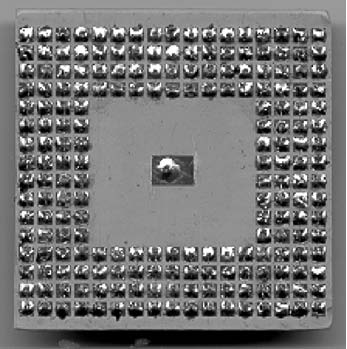
\includegraphics[width=0.40\textwidth]{Aplicacion/foto-ebg-alrededor-antena.pdf}}
	\hspace{30pt}
	\subfigure[Antena rodeada por un escalón de sustrato,]{
		\label{fig:escalon-sustrato}
		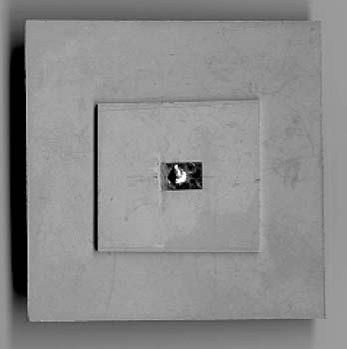
\includegraphics[width=0.40\textwidth]{Aplicacion/foto-escalon-alrededor-antena.pdf}}
	\caption{Fotos de diseños de antenas parches con limitadores a la propagación de onda de superficie \cite{Yang:EBGAntennas}.}
	\label{fig:limitadores-ondas-superficie-yang}
\end{figure}

Las primeras estructuras EBG utilizadas con estos fines consistían en arreglos de agujeros cilíndricos en el sustrato que, debido a la periodicidad que presentaban para las ondas de superficie, daban lugar a un comportamiento de filtro, presentando una banda prohibida. La dificultad para la fabricación de este tipo de sustratos dio lugar a la búsqueda de estructuras de banda prohibida de mayor facilidad de uso. En 1999, Sievenpiper presentó, en sus tesis doctoral \cite{Sievenpiper:Thesis}, una estructura que denominó HIS (\textit{High Impedance Surface}, superficie de alta impedancia), que además de cumplir con las características de un conductor magnético para un rango de frecuencias \cite{Sievenpiper:HIESForbiddenBand} y de ser de fácil fabricación con tecnología \textit{microstrip}, poseía también una banda prohibida electromagnética para las ondas de superficie \cite{Marcela:Tesis}. Esta estructura, consistente en parches metálicos dispuestos sobre un sustrato, y unidos al plano de tierra, ubicado en la cara opuesta del mismo, a través de vías metálicas, redujo ampliamente los costos y la dificultad de fabricación. Pocos años más tarde, debido a que en algunos casos el uso de vías retrasa la fabricación de circuitos \textit{microstrip}, surgieron estructuras de banda prohibida uniplanares, con características similares, aunque con anchos de banda prohibida más reducidos.

Para el presente trabajo, estas estructuras se ubicarán entre dos antenas microstrip, alineadas según distintos criterios, a fin de comparar el diagrama de radiación y el acoplamiento mutuo con el que se logra con el mismo arreglo radiante, pero sin el uso de EBG entre ellas.

% Coccioli, Yang, Itoh, intro historica.
\section{Criterios y técnicas utilizados para aumentar el ancho de banda de las antenas microstrip}
\label{sec_aumento_bw}
%%%%
Para poder utilizar las técnicas de blindaje contra ondas de superficie utilizando metamateriales, como las descriptas antes, es necesario que el ancho de la banda prohibida de la estructura EBG resulte mayor al ancho de banda de la antena. Es debido al alto valor del factor Q (y por tanto, bajo ancho de banda) de las antenas \textit{microstrip} rectangulares el motivo por el que el uso de estructuras EBG es factible.

Considerando que el objetivo del presente trabajo no es meramente la determinación de la posibilidad o no del uso de EBGs para disminuir el acoplamiento mutuo de antenas \textit{microstrip}, sino que se pretende describir y caracterizar someramente el comportamiento del metamaterial en cuestión, resulta necesario utilizar antenas de ancho de banda mayor a las \textit{microstrip} convencionales que se describieron en el capítulo \ref{cap_intro_electro}. De esta manera, sería posible encontrar los límites de uso y la tolerancia a variación de tamaños sin variación de la estructura EBG utilizada, lo que flexibiliza el trabajo de diseño.

Existen numerosas técnicas que permiten aumentar el ancho de banda de las estructuras radiantes de tecnología \textit{microstrip}. Como se explicó antes, una técnica común consiste en aumentar al ancho del sustrato, o cambiarlo por otro de constante dieléctrica menor. Debido a que la modificación de cualquiera de los dos parámetros condicionaría sustancialmente el comportamiento de las ondas de superficie generadas sobre el sustrato, se decidió que resultaba importante independizarlos del análisis.

En otros casos, se ha propuesto la modificación de la geometría del elemento radiante, descartando el tradicional parche rectangular por figuras con formas de U o de E, o por formas geométricas con aperturas radiantes embebidas \cite{Yang:EBGAntennas}. Para las mediciones de este trabajo se consideró, y finalmente se descartó, el uso de antenas \textit{microstrip} de tipo moño (\textit{bow-tie}), que presentan una transición geométrica suave, intuitivamente apta para las necesidades presentadas. Entre las dificultades que ofrece, está su principio de funcionamiento, comparable al de un dipolo, y requiriendo, por tanto, una alimentación en modo diferencial, lo que obligaría a realizar un diseño de un balún \textit{microstrip}, lejano a las pretensiones del trabajo.

Otra técnica común consiste en diseñar conjuntos de elementos que resuenan a distintas y frecuencias, acoplados capacitivamente, denominados estructuras multi-resonantes. Si las distintas frecuencias de resonancia están lo suficientemente cerca unas de otras, se logra un efecto de continuidad, aumentando notoriamente el ancho de banda. En muchos casos, y debido a los costos cada vez más despreciables de la fabricación de circuitos multicapa, los elementos resonantes se ubican apilados, generando un acoplamiento capacitivo máximo entre ellos. Para el caso de las pruebas que se requieren hacer para validar y caracterizar el comportamiento de las estructuras EBG, elementos radiantes coplanares con el parche activo resonante resultan suficientes.

La estructura propuesta consiste en un parche rectangular, ubicado sobre un sustrato de FR4, de comportamiento resonante en una frecuencia aproximada de 2.4 GHz, y ubicado entre dos rectángulos \textit{microstrip} pasivos iguales, de un largo establecido de forma que la frecuencia de resonancia de los mismos resulte ligeramente diferente a la del parche activo. La distancia entre estos elementos de carga y la antena original debe ser tal que el acoplamiento sea notorio, requisito que presenta complejidades \cite{Kumar:radiating} debido a que los parches deben estar ubicados frente a los bordes no radiantes de la antena para evitar reducir el espacio utilizado por la estructura EBG con la que compartirán sustrato. En la figura \ref{fig:antena-propuesta-con-ebg} se puede observar el arreglo final de elementos. Se debe destacar que la elección de que ambos parches posean las mismas propiedades geométricas se debe a la búsqueda de la máxima simetría par para simplificar el análisis de la estructura, aún cuando esta elección merme la flexibilidad del diseño de banda ancha.

\begin{figure}[h]
	\centering
	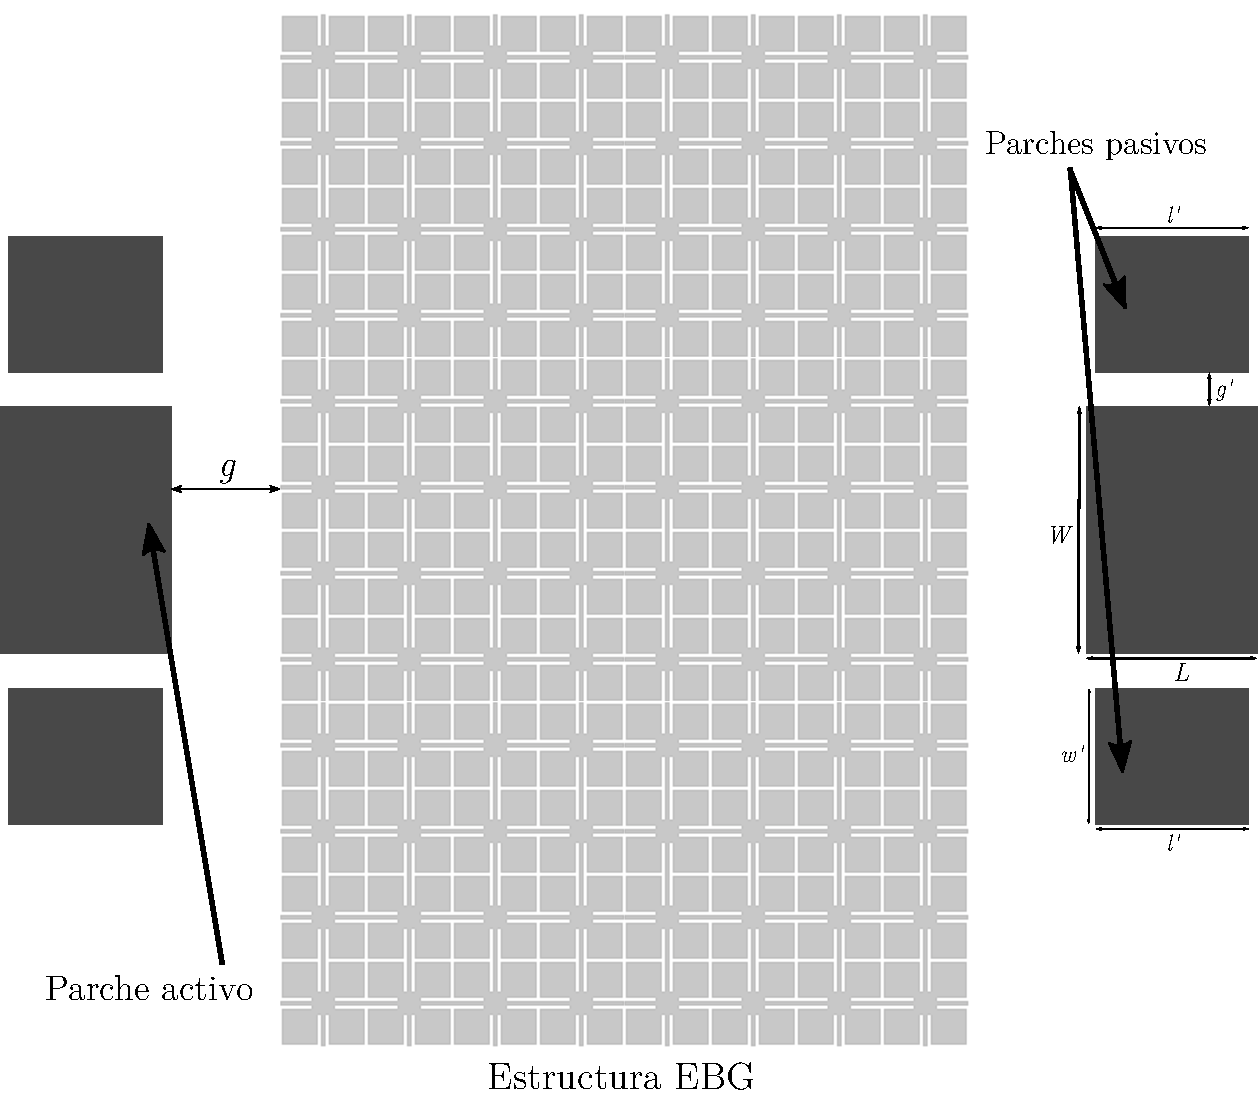
\includegraphics[width=0.9\textwidth]{Aplicacion/estructura-antenas-ebg.pdf}
	\caption{Estructura propuesta para la caracterización del efecto de EBGs sobre antenas microstrip.}
	\label{fig:antena-propuesta-con-ebg}
\end{figure}


Los parches rectangulares, al igual que en el desarrollo del análisis de estructuras EBG, están acoplados al elemento activo mediante lo que puede modelarse como una red $\pi$ de capacitores (acoplamiento capacitivo) \cite{Kumar:Non-radiating}, similar a mostrada en la figura \ref{fig:acoplamiento-capacitivo-modelo}, donde los denominados \textit{pixeles} deben ser reemplazados por los parches propiamente dichos. En términos generales, los parámetros que modificarán la impedancia de entrada y que, por lo tanto, afectarán al ancho de banda, son la distancia entre el resonador activo y los pasivos ($g$), la longitud de los parches acoplados ($l'$) y la posición del punto de alimentación \cite{Kumar:Non-radiating}.

La existencia de estos parches, que pueden considerarse como de carga, implican una modificación de la impedancia de entrada para distintas frecuencias.

Si los parches pasivos poseen dimensiones muy disímiles al parche activo central, las frecuencias de resonancia de los elementos estarán tan alejadas entre sí que es posible un análisis simplificado del comportamiento: A bajas frecuencias, los rectángulo pasivos no resuenan ni se acoplan visiblemente al parche activo. A medida que la frecuencia de trabajo aumenta, los mismos comienzan a acoplarse, adoptando un comportamiento capacitivo, al mismo tiempo que debido a que forman un paralelo con la carga impuesta por la resistencia de radiación, disminuyen el valor de la resistencia de entrada. Una vez que los parches resuenan, logrando que se presente la mínima resistencia de entrada, obtienen un comportamiento de carácter inductivo, hasta que nuevamente, a altas frecuencias, dejan de tener injerencia palpable sobre el valor de la impedancia de entrada. La variación de la distancia entre los parches da lugar a que estos efectos se vuelvan más o menos plausibles, en función del acoplamiento capacitivo \cite{Kumar:Non-radiating}.

Cuando los parches pasivos poseen geometrías similares a la del parche original, el problema resulta más complejo, debido a que no puede analizarse la resonancia de cada elemento por separado sin considerar la carga que los demás ejercen sobre él. Debido a que, a fin de aumentar el ancho de banda, todos los parches deberán tener geometrías similares, resulta necesario realizar simulaciones numéricas que permitan predecir el comportamiento.

%%%%
\section{Diseño de la antena \textit{microstrip}}
\label{sec_disenio_microstrip}
%%%%
El diseño de la antena microstrip consta de dos etapas: La primera de ellas consiste en el uso de los modelos teóricos de la sección \ref{subsec_antenas_microstrip} para diseñar una antena \textit{microstrip} para la frecuencia deseada; y la segunda consiste en la modificación del diseño, para lograr aumentar su ancho de banda de forma notoria, lo que inevitablemente genera cambios en la frecuencia de resonancia y valor de ROE de la antena. Estas variaciones se pueden predecir mediante simulación, lo que obliga a un proceso iterativo de corrección y simulación para lograr las características deseadas, que en los programas comerciales suele estar automatizado, bajo el nombre de optimización.

Se debe calcular, en primer lugar, un valor tentativo del ancho W de la antena (con W según la figura \ref{fig:antema-microstrip-inset} a)), teniendo en cuenta que un mayor ancho W da lugar a una menor resistencia de entrada $R_{in}$. Una fórmula empírica está dada por \cite{Barthia:Handbook}, y para una frecuencia de resonancia de unos 2.42 GHz y sustrato FR-4 de 1.6 mm de espesor, resulta:

\begin{align}
W = \frac{c_0}{2 f_r} \sqrt{\frac{2}{\epsilon_r+1}} = 37.35\; mm
\end{align}

Obtenido el ancho aproximado, se puede calcular la permitividad eléctrica eficaz, $\epsilon_{eff}$, de la ecuación \ref{cte-diel-efectiva-microstrip}, que obtiene el valor 4.17. Esto permite, conociendo la frecuencia de resonancia buscada, calcular la longitud efectiva de la línea de transmisión, como:

\begin{align}
	L_{eff} = \frac{c_0}{2 f_r \sqrt{\epsilon_{r_{eff}}}} = 30.32\; mm
\end{align}

Dado que $L_{eff} = L + 2 \Delta L$, a partir del cálculo de $\Delta L$, que cuantiza el efecto del \textit{fringing} sobre la frecuencia de resonancia, usando la expresión \ref{eq:deltaL-antena-microstrip}, que resulta en 0.74 mm, se puede saber el valor de L a utilizar ($L = L_{eff} - 2 \Delta L$), que es de 28.85 mm.

Además de la antena, debe diseñarse también la alimentación de la misma. De entre las múltiples formas de alimentación de una antena \textit{microstrip} \cite{Barthia:Handbook}, la seleccionada por su facilidad de fabricación es la que consiste en una línea de la misma tecnología, que vincula a un conector en el borde de la placa con el parche, esquematizado antes en la figura \ref{fig:antema-microstrip-inset}. En particular, es importante que la impedancia característica de la línea \textit{microstrip} utilizada sea de $50\;\Omega$, para lo que debe seleccionarse con cuidado su ancho, en función de la altura del sustrato y la permitividad del dieléctrico. Según las expresiones que se pueden hallar en el Apéndice B de \cite{Barthia:Handbook}, el ancho necesario para obtener una impedancia de $50\;\Omega$ es de aproximadamente 3.1 mm.

Conocidos estos valores, resta determinar el \textit{inset} que debe aplicarse para obtener una impedancia de entrada de 50 $\Omega$, a fin de lograr adaptación. Para esto, se debe utilizar la curva de la figura \ref{fig:antema-microstrip-inset} b), conociendo previamente el valor de la impedancia sobre el borde del parche rectangular. A partir de las expresiones de la parte real de la admitancia, o conductancia, obtenidas de \cite{Balanis:Theory} y mostradas en las ecuaciones \ref{eq:conductancia-microstrip-balanis} (donde $J_0$ es una función de Bessel del primer tipo de orden cero), la resistencia de entrada resulta $R_{in} = 1/[2(G_1 \pm G_{12})]$. A partir de este valor, la consulta a la gráfica permite deducir que el valor de \textit{inset} requerido es de aproximadamente 10.73 mm.

\begin{align}
	\label{eq:conductancia-microstrip-balanis}
	G_1 &=& \frac{1}{\pi \eta_0} \int_0^\pi \left[ \frac{\sin \left( \frac{k_0 W}{2} \cos \theta \right) }{\cos \theta}\right]^2 \sin^3 \theta d\theta \\
	G_{12} &=& \frac{1}{120 \pi^2} \int_0^{\pi} \left[ \frac{\sin \left( \frac{k_0 W}{2} \cos \theta \right) }{\cos \theta}\right]^2 J_o(k_0 L \sin \theta) \sin^3 \theta d\theta
\end{align}

El siguiente paso consiste en describir geométricamente la estructura calculada para el uso de un software de simulación que permita optimizar los parámetros, en vistas de que la frecuencia de resonancia sea 2.41 GHz, y que el parámetro $S_{11}$, correspondiente al puerto de alimentación, sea tan pequeño como sea posible. Es importante aclarar que el agregado de los parches de carga y de la estructura EBG modificará la frecuencia de resonancia, y que este análisis se realiza en miras de comprender los cambios que se producen sobre la antena original, y confirmar el aumento de ancho de banda mediante la técnica mencionada antes.

%Comentar resultados de simulación. Imagenes de la misma.%
% Las simulaciones quedaron en mi pc: Metamateriales/Simulaciones/Simo3-CST/Celdas Unitarias / Celdas Unitarias Consideradas / UCPBG / Simulaciones para medicion / UnParche-SinCarga-SinEBG.cst

% Comparar:
% -varios insets, mismo alto y largo total de antena
% -mostrar qué pasa cuando varía el largo de la antena, para un inset fijo
% -mostrar qué pasa cuando varía el alto de la antena, apra inset fijo.

% Simular la optimización y poner los resultados.
% Incluir farfields!

Finalizado el diseño analítico del parche único, resta considerar el uso de los parches \textit{microstrip} acoplados capacitivamente al parche activo principal. Para ello, se realizaron sucesivas simulaciones en el software de simulación CST Microwave Studio, realizando una optimización para obtener el mayor ancho de banda posible dentro del rango de interés. Los parches deben ser de un largo similar a la antena, aunque ligeramente diferente, para aumentar el ancho de banda. Por otro lado, se eligió que fueran simétricos, a fin de no aumentar la anisotropía del problema.

% Acá seguramente hay que hacer aun las simulaciones. los valores de la antena oroginal no están 100% definidos, y algo pueden cambiar en la optimización. La idea es fijar un valor, mostrar cómo cambia, y luego optimizar.

%% Poner resultados

El diseño de un único parche cargado no equivale al problema completo, aunque sí permitirá luego comparar el comportamiento del parche aislado con el que se obtiene cuando se ubica otra antena \textit{microstrip} rectangular cerca, y cuando se utilizan estructuras EBG para intentar aislarlas.

Para poder estudiar este problema, será necesario comprender cómo se comporta un conjunto de dos antenas \textit{microstrip} sin estructuras entre ellas, separadas una distancia adecuada para que los efectos de acoplamiento mutuo resulten visibles.

%% COMO ES ESA DISTANCIA??

% Simular, incluyendo farfield.

% PONER FOTO
% Poner resultados finales

% Condiciones de borde: LIbroSinNombre, pagina 398.
%%%%
\section{Elección del metamaterial}
\label{sec_eleccion}
%%%%
% Cantidad de celdas minima: Bouali, Aguili, impreso.
% Pedir que bw del metamaterial sera mayor al de la antena
% Mirar el analisis de Coccioli, Yang, Itoh, pag 2126
% ¿criterio para la distancia? IMPORTANTE!!!!!
%%%%

\section{Estudio del efecto de la distancia sobre el ancho de banda}
\label{sec_efecto_distancia}
%%%%
%Coccioli, Yang, Itoh, pag 2127
% Iluz, Shavit, pag 1448

Finalmente, es necesario agregar las estructuras EBG para observar el efecto que producen en el arreglo de antenas. Para ello, en primer lugar se debe reducir el efecto que las estructuras ejercen sobre cada uno de los parches por separado, para lo cual también se realizó un conjunto de simulaciones, donde las estructuras se ubicaron a distintas distancias de la antena.

\section{Estudio del efecto sobre el acoplamiento mutuo}
\label{sec_estudio_acoplam_mutuo}
%%%%
Establecida la distancia adecuada, es posible ahora incorporar a la simulación las estructuras EBG para observar el efecto sobre el acoplamiento mutuo. Se debe tener en cuenta que la cantidad de celdas unitarias debe ser suficiente para lograr el efecto deseado.


% Ondas de superficie se proparagan por plano E? Pagina 132. Rahmat, lbro,.
% Pagina 138. Rahmat.
% Efecto según la orientacion de parches. ABidin, Tesis, Pagina 37.
% Algo se puede ver en Assimonis, Yioultsis, Antonopoulos
%%%%


% Ver que overall las conclusiones son similares a Islam,Alam.
